\documentclass[a4paper,10pt]{article}
\usepackage[T1]{fontenc}
\usepackage[utf8]{inputenc}
\usepackage{lmodern,textcomp}
\usepackage[margin=2.2cm]{geometry}
\usepackage{amsmath,amssymb,siunitx,booktabs,graphicx,tabularx,array,enumitem,xcolor,fancyhdr,float,fancyvrb}
\usepackage[colorlinks=true,linkcolor=blue!50!black,urlcolor=blue!50!black]{hyperref}
\setlength{\parindent}{0pt}
\setlength{\parskip}{4pt}
\setlength{\headheight}{14pt}
\renewcommand{\arraystretch}{1.2}
\renewcommand{\tabularxcolumn}[1]{>{\raggedright\arraybackslash}p{#1}}
\setlist{nosep,leftmargin=*}
\newcommand{\file}[1]{\nolinkurl{#1}}
\newcommand{\todo}[1]{\textcolor{red}{[TODO: #1]}}
\sisetup{per-mode=symbol}
\pagestyle{fancy}\fancyhf{}
\fancyhead[L]{34870 Electroacoustics}
\fancyhead[R]{Loudspeaker project --- System D}
\fancyfoot[L]{Group 10}
\fancyfoot[R]{\thepage}
\graphicspath{{../figures/}{Project/figures/}{../ltspice/}{Project/ltspice/}}
% compiles both locally (from Project/report) and in Overleaf (from the repo root)
\newcommand{\res}[1]{\IfFileExists{#1}{\input{#1}}{\input{Project/report/#1}}}
\newcommand{\verbfile}[1]{\IfFileExists{../data/dsp/#1}{\VerbatimInput[fontsize=\footnotesize]{../data/dsp/#1}}{\VerbatimInput[fontsize=\footnotesize]{Project/data/dsp/#1}}}
\res{results_task1.tex}
\res{results_design.tex}

\begin{document}
\begin{center}
{\Large\bfseries Loudspeaker project --- three-way system D}\\[5pt]
34870 Electroacoustics\\[4pt]
Group 10: Louis Andrianne, Sophie Kimura, Mads Rudolph\\[4pt]
System D (shared with Group 4): Scan-Speak 26W/8534G00 woofer box + DALI Spektor 2 (S/N 7446912 -- L)
\end{center}
\thispagestyle{fancy}

\begin{center}
\fbox{\begin{minipage}{0.92\linewidth}\small
\textbf{Status (branch \file{project-solution}).} Tasks 1 and 2 are designed and simulated from the
Lab D/E data; Tasks 3 and 4 are prepared (coefficients, parts list, test procedure) and wait for lab
time. Every number in this report is written by the scripts (\file{results_task1.tex},
\file{results_design.tex}), so rerunning them updates the text. How to rerun everything:
\file{Project/README.md}, section ``Solution branch''.
\end{minipage}}
\end{center}

\section{System and plan}
The system follows Figure~1 of the guide. Amplifier channel~1 is fed by MiniDSP output~1 (digital
low-pass) and drives the woofer box. Channel~2 is fed by output~2 (digital high-pass) and drives the
passive board, which splits it into a low-pass for the midrange and a high-pass with an L-pad for the
tweeter. Our design:

\begin{center}
\begin{tabular}{ll}
\toprule
Woofer box & one vent, $L = \SI{160}{mm}$ ($f_B = \SI{\bfBA}{Hz}$), no extra filling \\
Digital crossover & \xalignDig\ at \SI{\xfcDig}{Hz} (two identical Butterworth biquads), woofer gain \SI{\xgWoof}{dB} \\
Midrange low-pass & \xtopoMid: series \xMidLa, shunt \xMidCa \\
Tweeter high-pass & \xtopoTw: series \xTwCa, shunt \xTwLa; L-pad $R_s = $ \xTwRs, $R_p = $ \xTwRp \\
Polarity & all three units normal (+) \\
Acoustic crossovers & \SI{\xxWM}{Hz} (woofer/mid) and \SI{\xxMT}{Hz} (mid/tweeter) \\
Result (simulated) & \SIrange{150}{15000}{Hz} within \SI{\xspreadOn}{dB} on axis, \SI{\xspreadOff}{dB} at $30^\circ$ ($1/6$ octave) \\
\bottomrule
\end{tabular}
\end{center}

The tools behind it, all in \file{Project/}:
\begin{itemize}
\item \file{matlab/export_systemD.m}: the Lab D/E data into LTspice text files and CSV.
\item \file{ltspice/task1/}: the woofer-box model fitted to Lab D (\file{box_model.py}) and its
  LTspice circuit (\file{Task1_WooferBox.asc}, verified against the closed form).
\item \file{design/xover.py}: the complete chain (biquads, passive ladders loaded by the measured
  $Z_i$, measured TFs, sum) with a search over Appendix~1 values; \file{design/design.json} holds
  the design.
\item \file{ltspice/System_D_design.asc}: the same design in LTspice, verified against \file{xover.py}
  at all 412 measured frequencies.
\item \file{app/}: \emph{Crossover Studio}, an interactive version of the whole model in the browser.
\end{itemize}

\section{Task 1: Low-frequency tuning of the woofer box}
\subsection{Thiele--Small parameters (Lab D)}
The free-air and closed-box impedances were fitted together with one circuit (Lecture~7): $R_E$ from
the multimeter, $S_D$ from the data sheet, and $Bl$, $M_{MD}$, $C_{MS}$, $R_{MS}$, $L_E$ free. Free air
loads both sides of the cone with an unbaffled piston, the closed box loads the front with a baffled
piston and the back with $C_{AB} = V_B/\rho c^2$. The closed box is what pins down $C_{MS}$ (and so
$V_{AS}$), because $S_D$ is fixed.

\begin{center}
\begin{tabular}{lccc}
\toprule
 & Lab D, \file{analyse_labD.m} & Lab D, circuit fit & Data sheet$^\ast$ \\
\midrule
$f_S$ (Hz) & 22.7 & \bfS & 22.9 \\
$Q_{MS}$ & 9.95 & \bQMS & 9.1 \\
$Q_{ES}$ & 0.511 & \bQES & 0.41 \\
$Q_{TS}$ & 0.486 & \bQTS & 0.39 \\
$V_{AS}$ (L) & 213 & \bVAS & 165 \\
$Bl$ (T\,m) & -- & \bBl & 10.1 \\
$M_{MS}$ (g) & -- & \bMMS & 50.5 \\
$C_{MS}$ (mm/N) & -- & \bCMS & 0.95 \\
$R_E$ ($\Omega$), $L_E$ (mH) & 5.7, -- & 5.7, \bLE & 5.7, -- \\
\bottomrule
\end{tabular}\\[2pt]
{\footnotesize $^\ast$ $f_S$, $Q$s and $V_{AS}$ computed from the data sheet's $M_{MS}$, $C_{MS}$, $Bl$, $R_{MS}$ and $S_D = \SI{350}{cm^2}$.}
\end{center}

Our driver is softer than the data sheet ($V_{AS}$ about 25\,\% larger) and has less motor
($Q_{ES}$ 0.50 against 0.41). Both shifts point the same way as a sample-to-sample spread plus a
suspension that has loosened with use. The fit reproduces both curves (Figure~\ref{fig:zfit});
the remaining misfit is the semi-inductive voice coil above \SI{150}{Hz}, which does not matter
below the crossover.

\subsection{LTspice analogy circuit of the box}
The circuit (Figure~\ref{fig:task1sch}) uses the impedance analogy in all three domains, as in
Lecture~7, slide~27. In the acoustic domain the cone's volume velocity $U_D = S_D u$ flows through the
box network and then through the front radiation impedance. The box network is $C_{AB}$ in parallel
with a leak $R_{AL}$ and with the vent branch $M_{AP} + R_{AP}$. The current through the vent branch is
$U_P$, and the far field is $p \propto j\omega\rho\,(U_D - U_P)/2\pi r$. One \file{.step} runs the
plugged box and the three measured vent lengths; a fifth step is free for trying other values.
\file{gen_box_ltspice.py --verify} confirms LTspice equals the closed form to $2\cdot10^{-4}$ in every step.

Two findings from fitting the three vented impedance curves:
\begin{itemize}
\item \textbf{The vent does not follow the tube formula.} With $M_{AP} = \rho(L + 1.46a)/\pi a^2$ and
  $a = \SI{32.5}{mm}$, the tuning should move from 23.4 to \SI{19.8}{Hz} between $L = 160$ and \SI{240}{mm}.
  The measurement moves half as much. We therefore fitted one effective $M_{AP}$ per length:
  \bMAPA, \bMAPB, \bMAPC~kg/m$^4$ against \bMAPformulaA, \bMAPformulaB, \bMAPformulaC\ from the
  formula ($f_B$ = \bfBA, \bfBB, \bfBC~Hz). Likely causes: the length we noted is the telescope's
  extension, not the acoustic length, or the inner tube is narrower than \SI{65}{mm}. \todo{measure
  both vents' inner diameters and the telescopic range on the box.}
\item \textbf{The losses come with the open vent.} With the vents plugged, the box is practically
  lossless (the closed-box peak, \SI{121}{\ohm}, needs no leak). With a vent open, the curves need
  $Q_L = \bQL$ and $Q_P = \bQP$. That is the signature of port losses, not of a leaky box, so the
  plugged and vented configurations keep separate losses.
\end{itemize}

\subsection{Validation against the near-field measurements}
Figure~\ref{fig:nf} compares the near field predicted from the impedance fit, $p \approx j\omega\rho
U/\pi a$ at the centre of each opening, with the measured cone and vent pressures in Pa/V. Nothing in
this figure is fitted. Levels agree within 2--3\,dB, the vent and cone curves cross where measured,
and the cone notch falls \SIrange{1}{2}{Hz} above the measured one. Above about \SI{60}{Hz} the vent
microphone picks up the cone, so the measured vent curve stops falling there. Below \SI{120}{Hz} the
room modes of room 026 add ripple the model does not have.

\subsection{Chosen tuning}
Figure~\ref{fig:tuning} and the table compare the options. Because $Q_{TS}$ is high (0.47) and
$V_{AS}$ much larger than $V_B$ ($\alpha = 2.3$), no standard alignment from Lecture~8 can be
reached. More importantly, $f_3$ hardly depends on the tuning: every $f_B$ from 22 to \SI{30}{Hz}
gives $f_3 \approx \SI{33}{Hz}$, and only the ripple grows.

\begin{center}
\begin{tabular}{lccc}
\toprule
Configuration & $f_B$ (Hz) & $f_3$ (Hz) & ripple (dB) \\
\midrule
Vents plugged (closed) & -- & \bfthreeCl & \brippleCl \\
One vent, $L = \SI{160}{mm}$ & \bfBA & \bfthreeA & \brippleA \\
One vent, $L = \SI{200}{mm}$ & \bfBB & \bfthreeB & \brippleB \\
One vent, $L = \SI{240}{mm}$ & \bfBC & \bfthreeC & \brippleC \\
$M_{AP} = 52$ (e.g.\ both vents) & 28.0 & 32.7 & +2.4 \\
\bottomrule
\end{tabular}\\[2pt]
{\footnotesize $f_3$ against the mean level at \SIrange{150}{300}{Hz}, half space, no room; ripple = highest point below \SI{150}{Hz}.}
\end{center}

\textbf{Choice: one vent at $L = \SI{160}{mm}$.} It extends $f_3$ from 37 to \SI{33}{Hz} at
\SI{1.8}{dB} ripple. Cone excursion between 25 and \SI{40}{Hz} drops to about a third of the closed
box's (Figure~\ref{fig:tuning}, bottom), so the woofer plays louder before it distorts. It is also a
configuration we actually measured, so the near field validates it directly. Opening both vents would
raise $f_B$ to about \SI{28}{Hz} for no gain in $f_3$ and +2.4\,dB ripple. Filling would add a few
hertz of extension but is not modelled reliably: we have no measurement with known filling. A
listening room adds its own low-frequency gain, so a mild hump of under \SI{2}{dB} in half space is
on the safe side.

\section{Task 2: Modelling the crossover filters}
\subsection{Measured data in LTspice}
\file{export_systemD.m} runs \file{Matlab2LTspice.m} on $Z_i$ of the midrange and tweeter (no distance)
and on the Lab E $p/V$ of all three units, on axis and at $30^\circ$, all with $d = \SI{-1.15}{m}$. It
then gives every generator and label a unit suffix (\file{Vspkr_mid}, \file{Pout_tw}, \dots). The three
Lab E units were measured in one run, so their relative phase is real, and the same $d$ is applied to
all of them. \file{ltspice/units/Unit_*.asc} are the course template with our files, driven straight
from the source. LTspice reproduces the measured $|Z_i|$ and $p/V$ to \SI{0.04}{dB} and \SI{0}{\degree}
at its own frequency points (\file{gen_templates.py --verify}). The tweeter $Z_i$ starts at
\SI{99}{Hz} and its $p/V$ is noise below about \SI{120}{Hz}, which is irrelevant behind a high-pass.

\subsection{Choosing the crossover frequencies}
\begin{itemize}
\item \textbf{Woofer--midrange.} The \SI{26}{cm} woofer ($a = \SI{10.5}{cm}$) reaches $ka = 1$ at
  \SI{520}{Hz} and breaks up above \SI{1.5}{kHz}, where its $30^\circ$ curve falls apart. The midrange
  has its resonance at \SI{90}{Hz} and is flat from \SI{150}{Hz}. Hence \SIrange{300}{400}{Hz}.
\item \textbf{Midrange--tweeter.} The tweeter's resonance is at \SI{1.45}{kHz} (Lab D) and it is about
  \SI{10}{dB} more sensitive than the midrange. The midrange is still flat at $30^\circ$ up to about
  \SI{4}{kHz}. Hence \SIrange{2.5}{4}{kHz}, with an L-pad.
\end{itemize}

\subsection{Design method}
\file{design/xover.py} computes, for \SI{1}{V} at the MiniDSP input,
\[
p = p_w\,g_w H_{LP}(f)\,TF_w(f)\,B(f) + p_m H_{HP}(f)\,T_m(f)\,TF_m(f) + p_t H_{HP}(f)\,T_t(f)\,TF_t(f),
\]
where $H_{LP}$ and $H_{HP}$ are the MiniDSP biquads evaluated at $e^{j\omega T}$, $f_s = \SI{96}{kHz}$
(the strings are identical to \file{DigitalCrossover.m}'s, checked in MATLAB). $T_m$ and $T_t$ are the
passive ladders, solved with ABCD matrices and loaded by the measured $Z_i$. $TF$ is the Lab E data and
$B$ is the Task~1 box tuning (vented over plugged, from the fitted model), because Lab E had the vent
plugged. The design was found by coordinate descent over the allowed choices: $f_c$ in \SI{25}{Hz}
steps, BW2/LR4/BW4, woofer gain in \SI{0.5}{dB} steps, every passive value from Appendix~1, L-pad
values and polarities. The cost function combines:
\begin{itemize}
\item the RMS deviation of the $1/6$-octave-smoothed sum from flat, \SIrange{150}{15000}{Hz}, on axis
  plus half the $30^\circ$ value;
\item a penalty for cancellation, where the sum falls below the power sum;
\item penalties keeping the acoustic crossovers inside \SIrange{250}{600}{Hz} and
  \SIrange{2.2}{4}{kHz}, and the tweeter \SI{12}{dB} down at its resonance.
\end{itemize}
Without those penalties the search pulled the mid/tweeter crossover down to \SI{2}{kHz}. That is flat
on paper and wrong for the tweeter.

\subsection{Digital crossover woofer--midrange}
\xalignDig\ at \SI{\xfcDig}{Hz}: two identical Butterworth biquads ($Q = 0.707$) per output.
\file{DigitalCrossover.m} only gives Butterworth ($n = 4$ gives $Q = 0.541$ and 1.307), so the LR4
is made by running it with $n = 2$ and using that section twice. LR4 won over BW4 and BW2 because
the two outputs stay in phase through the crossover (Figure~\ref{fig:phase}). The woofer is
\SI{\xgWoof}{dB} relative to the mid/tweeter channel, which is the MiniDSP output~1 gain. Section~4.1
lists the coefficients.

\subsection{Passive crossover midrange--tweeter}
\begin{itemize}
\item \textbf{Midrange:} second-order low-pass, series \xMidLa, shunt \xMidCa ($1/2\pi\sqrt{LC} =
  \SI{\xfMidLC}{Hz}$). The driver's rising impedance (\SI{8.5}{\ohm} at \SI{2}{kHz}, \SI{13.6}{\ohm} at
  \SI{5}{kHz}) makes the filter peak slightly, which fills the midrange's own roll-off. That is why the
  electrical corner sits below the acoustic crossover.
\item \textbf{Tweeter:} second-order high-pass, series \xTwCa, shunt \xTwLa ($1/2\pi\sqrt{LC} =
  \SI{\xfTwLC}{Hz}$). The L-pad ($R_s$ = \xTwRs\ in series, $R_p$ = \xTwRp\ across the tweeter) takes
  about \SI{\xpadDB}{dB} off a \SI{4}{\ohm} tweeter and gives the filter a more resistive load around
  the tweeter's \SI{1.45}{kHz} resonance.
\item The acoustic slopes (filter $\times$ driver) cross at \SI{\xxMT}{Hz} in phase with normal
  polarity. With second-order electrical filters this is not the textbook ``invert the tweeter''
  case, because the drivers' own roll-offs and the offset between the acoustic centres add their own
  phase.
\item Amplifier channel~2 never sees less than \SI{\xZminAmp}{\ohm} (Figure~\ref{fig:filters}).
\end{itemize}

\subsection{Combined system response}
Figure~\ref{fig:system} shows the three contributions and the sum. On axis the
\SIrange{150}{15000}{Hz} response stays within \SI{\xspreadOn}{dB} (standard deviation
\SI{\xstdOn}{dB}); at $30^\circ$ within \SI{\xspreadOff}{dB}. The sum is \SI{3}{dB} above the power sum
exactly at both crossovers and never below it (Figure~\ref{fig:phase}): no cancellation anywhere. The
summing method is the one in the guide, series E sources with polarity factors, in
\file{System_D_design.asc} (Figure~\ref{fig:syssch}). LTspice and \file{xover.py} agree to
$<\SI{0.01}{dB}$ at every measured frequency.

\textbf{Tolerances.} A Monte Carlo of 400 runs varied the coils by $\pm5\,\%$, the capacitors by
$\pm10\,\%$ and the resistors by $\pm5\,\%$. The 95\,\% band of the sum is at most \SI{1.7}{dB} wide,
and coil resistance of 0.3--\SI{0.6}{\ohm/mH} changes it by at most \SI{0.45}{dB}
(Figure~\ref{fig:tol}). The design does not depend on lucky part values.

\section{Task 3: Implementing the crossovers}
\subsection{MiniDSP configuration}
Routing Input1$\to$Output1 and Input1$\to$Output2; on both outputs only Xover active (PEQ, Comp, FIR
bypassed). Paste into Output~1 $\to$ Xover $\to$ Advanced, then Process (file
\file{data/dsp/MiniDSP_woofer_out1.txt}):
\verbfile{MiniDSP_woofer_out1.txt}
and into Output~2 (\file{data/dsp/MiniDSP_midtw_out2.txt}):
\verbfile{MiniDSP_midtw_out2.txt}
Output~1 gain \SI{\xgWoof}{dB}, output~2 gain \SI{0}{dB}. The LTspice strings for the same filters are
in \file{data/dsp/LTspice_*.txt}.

\subsection{Passive filter board}
\begin{center}
\begin{tabular}{llll}
\toprule
Branch & Part & Value & Source \\
\midrule
Midrange & series inductor & \xMidLa & course basket (Appendix 1) \\
Midrange & shunt capacitor & \xMidCa & course basket \\
Tweeter & series capacitor & \xTwCa & course basket \\
Tweeter & shunt inductor & \xTwLa & course basket \\
Tweeter & L-pad series resistor & \xTwRs & course basket \\
Tweeter & L-pad shunt resistor (across the tweeter) & \xTwRp & course basket \\
\bottomrule
\end{tabular}
\end{center}
All values are single standard parts. Wiring order from the amplifier: tweeter branch $C \to$ node with
$L$ to ground $\to R_s \to$ tweeter with $R_p$ across it; midrange branch $L \to$ midrange with $C$
across it. Both branches start from amplifier channel~2, and both drivers are wired with normal
polarity. \todo{photo of the board, actual parts used, measured values if an LCR meter is available.}

\subsection{Anechoic measurement of the complete system}
Plan for the session: vents covered (the chamber is useless below \SI{125}{Hz} anyway).
\begin{enumerate}
\item Each unit alone through its full chain (MiniDSP active, other outputs muted): compare with the
  dashed unit curves of Figure~\ref{fig:system}.
\item All three together, $0^\circ$ and $30^\circ$: compare with the sum.
\item Woofer polarity flipped: there must be a deep notch at \SI{\xxWM}{Hz}. Tweeter flipped: a notch
  at \SI{\xxMT}{Hz}. This checks the wiring and the phase model in one go.
\end{enumerate}
\todo{measured vs.\ simulated, and what we changed.}

\section{Task 4: Listening test}
Procedure (IEC 60268-13 room, Lecture~10), planned:
\begin{itemize}
\item \textbf{Set-up:} the box on the floor at the standard position, the listener at \SI{2.5}{m} on
  axis at ear height near the tweeter. Level matched to \SI{80}{dB(A)} on pink noise with a sound
  level meter, so loudness does not decide the comparison.
\item \textbf{Comparison:} paired, A/B. A = the design, B = a variant (woofer gain $\pm\SI{2}{dB}$,
  tweeter $R_s$ one value up or down, vent plugged vs.\ open). The operator switches; the listener does
  not know which is which. Each pair is repeated with the order reversed.
\item \textbf{Material:} short excerpts (20--30\,s) with a male voice, acoustic guitar/piano, a track
  with steady bass, and pink noise.
\item \textbf{Questionnaire:} for each excerpt, preference A/B/none, and a 1--5 scale for bass
  quantity, midrange naturalness (voices), treble brightness, and overall. Free comments.
\item \textbf{Subjects:} at least 6, including people outside the group, with a short training round.
\end{itemize}
\todo{results, analysis (count preferences, mean scores per attribute) and the iteration it led to.}

\section{Conclusion}
\todo{after Tasks 3 and 4: final design, measured vs.\ simulated, what we would change.}

% ------------------------------------------------------------------ figures
\begin{figure}[p]
\centering
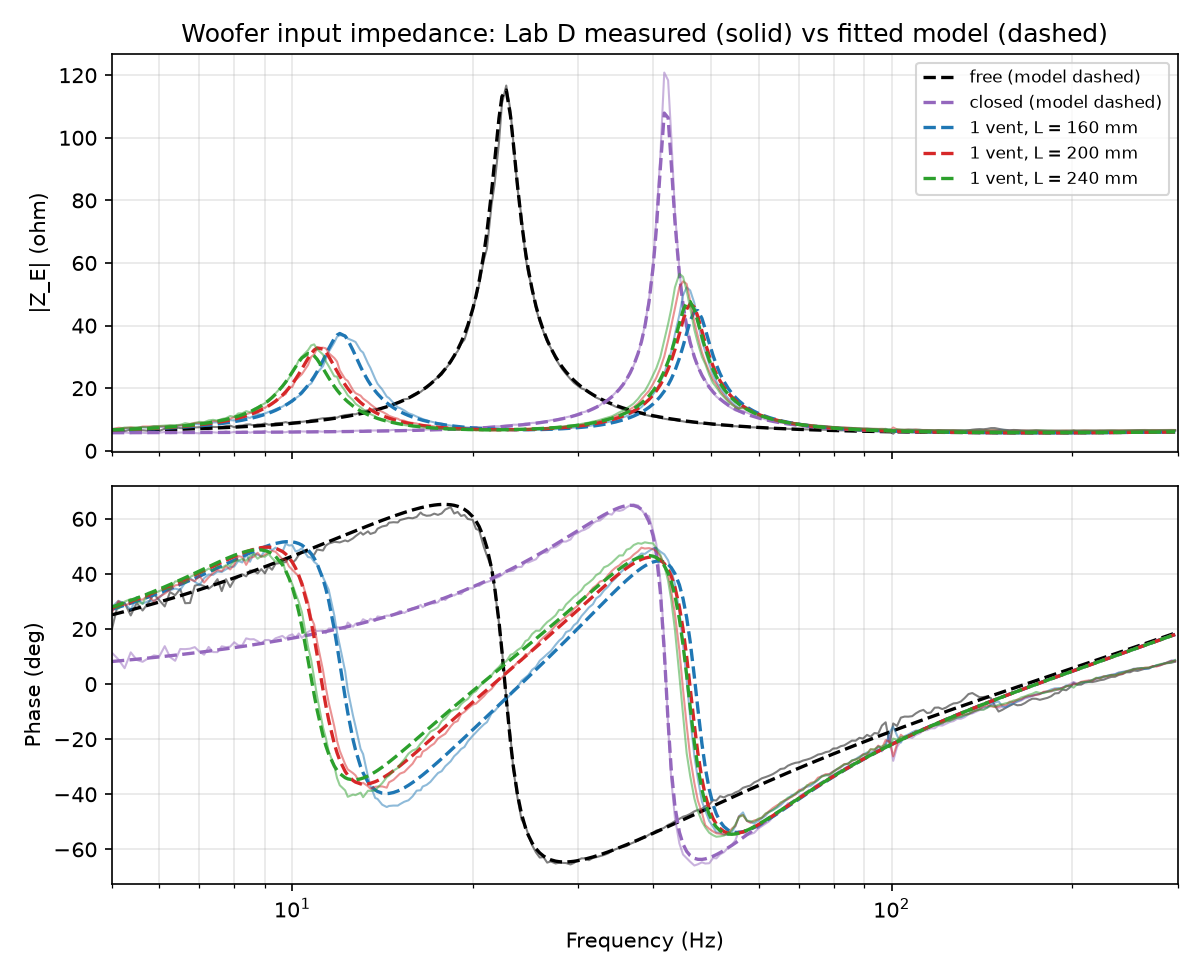
\includegraphics[width=0.85\linewidth]{task1_impedance_fit.png}
\caption{Woofer input impedance, Lab D measured (thin) and the fitted circuit (dashed): free air,
closed box and one vent at three lengths.}\label{fig:zfit}
\end{figure}

\begin{figure}[p]
\centering
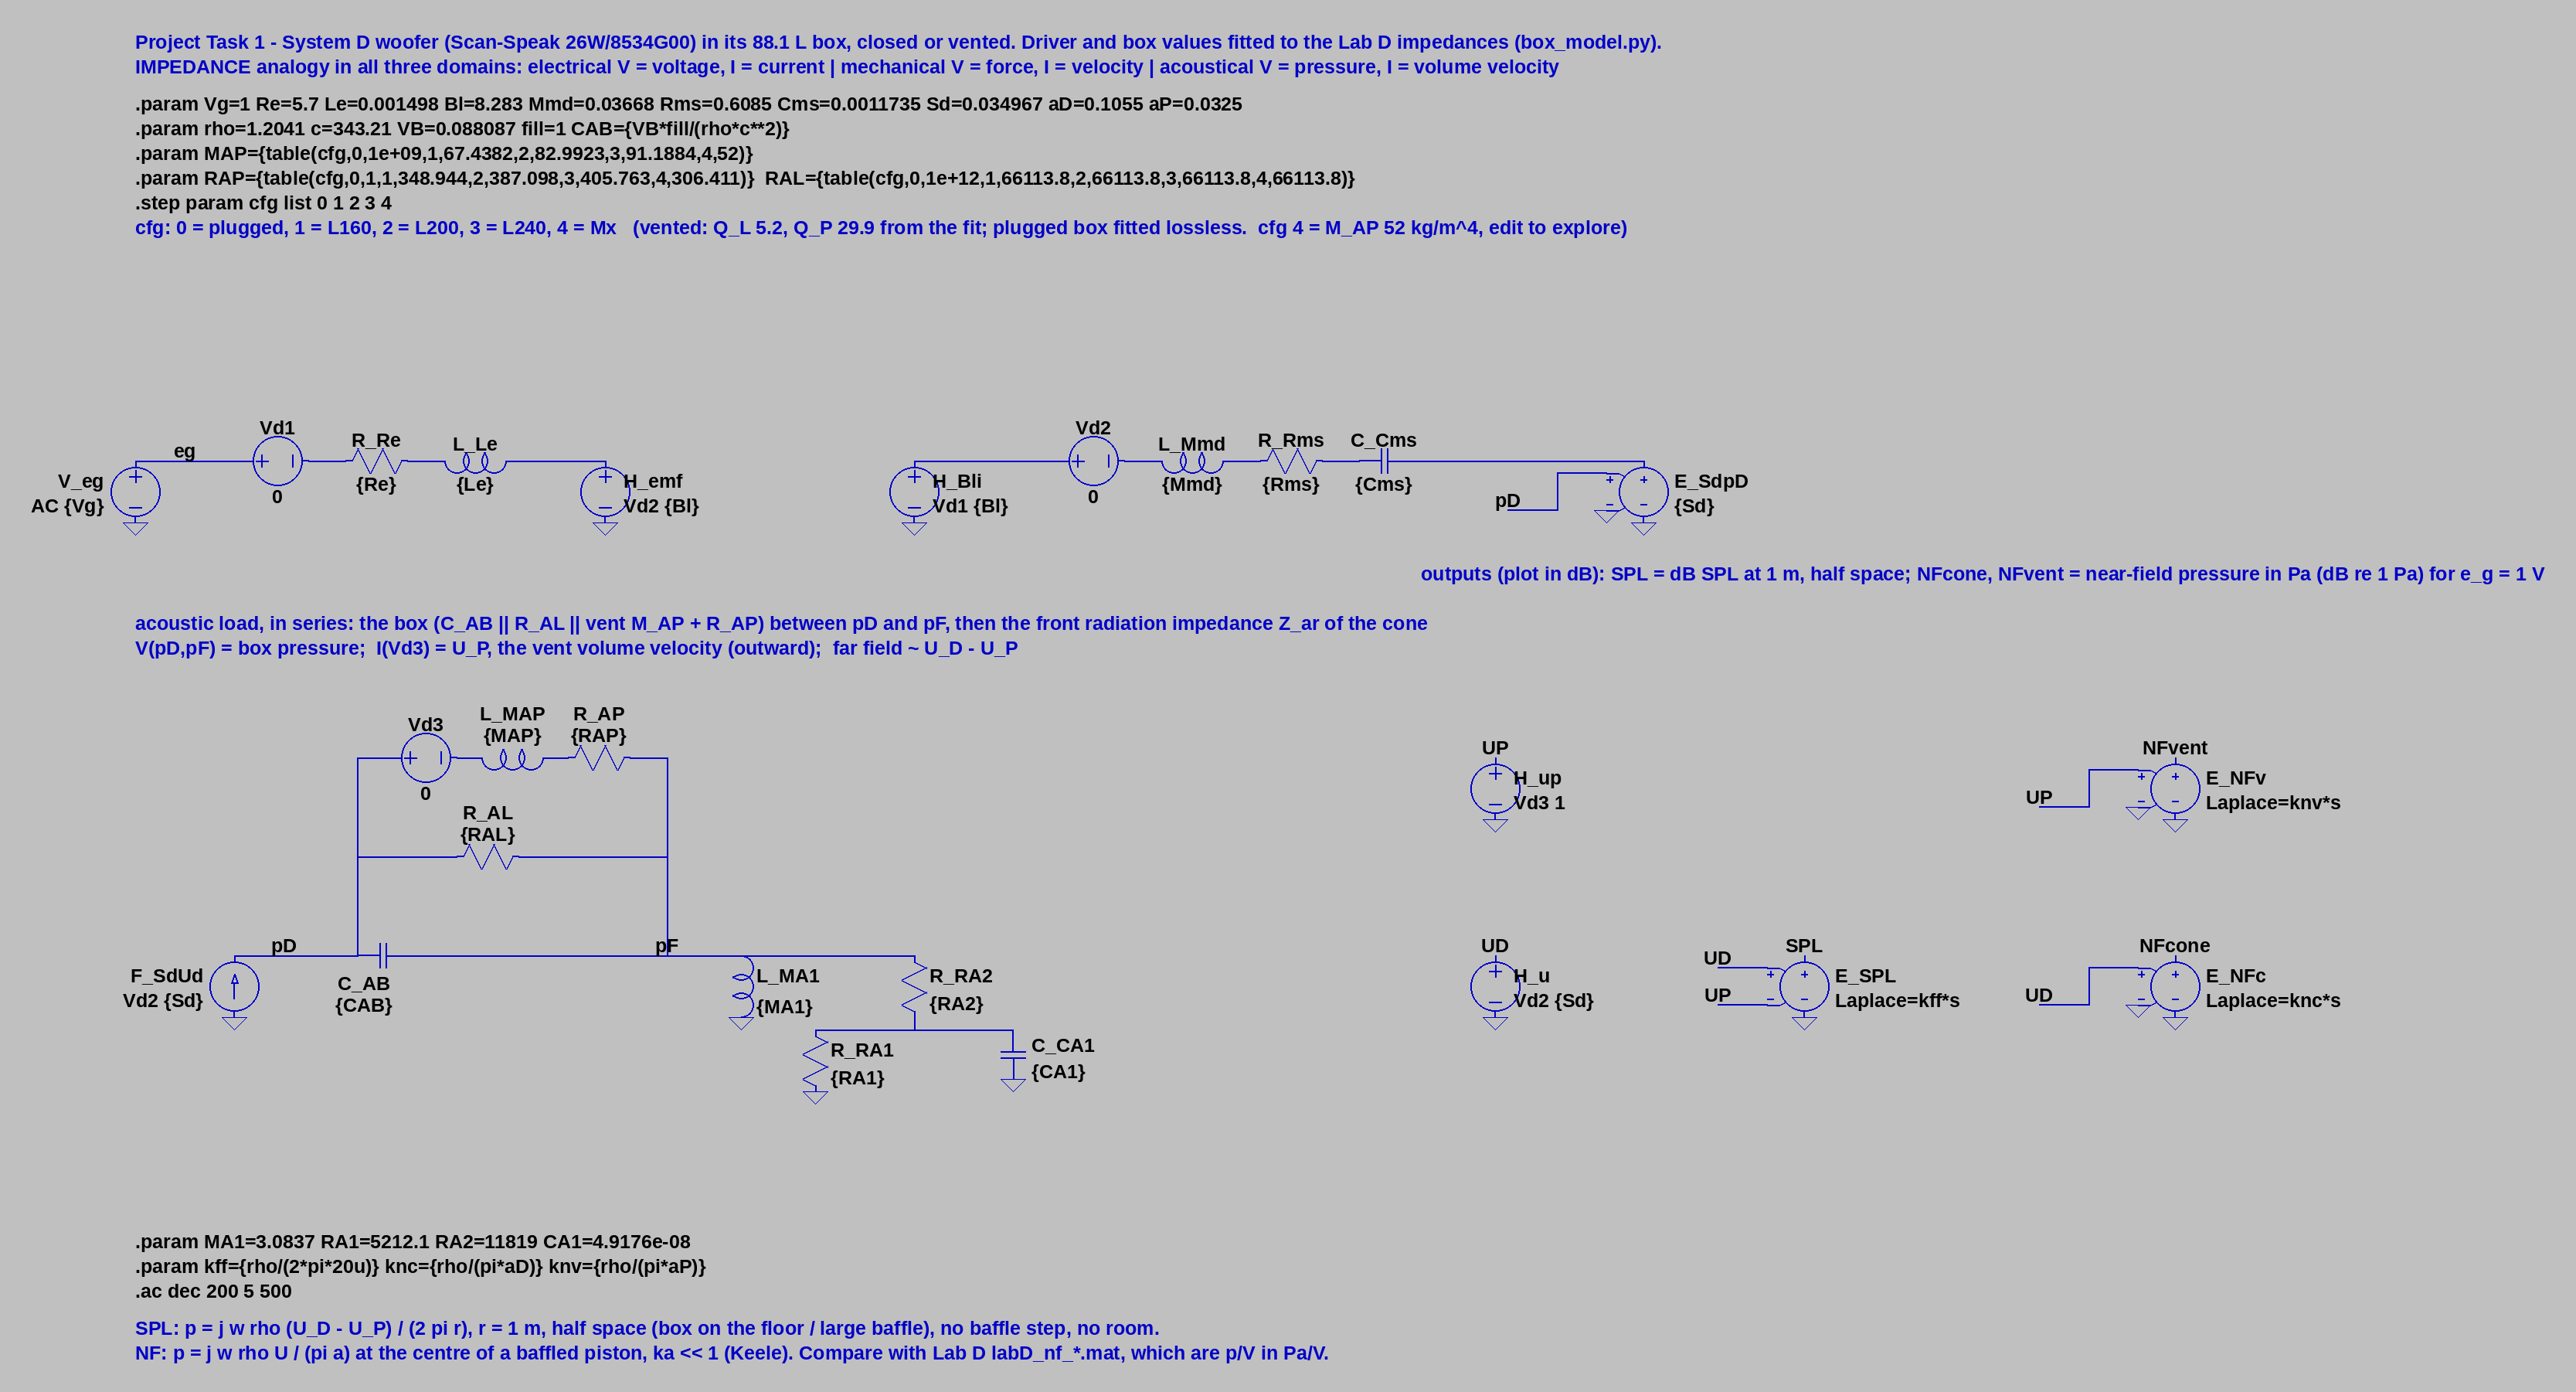
\includegraphics[width=\linewidth]{task1/preview/Task1_WooferBox.png}
\caption{\file{Task1_WooferBox.asc}: woofer, box and vent as an impedance analogy (LTspice).}\label{fig:task1sch}
\end{figure}

\begin{figure}[p]
\centering
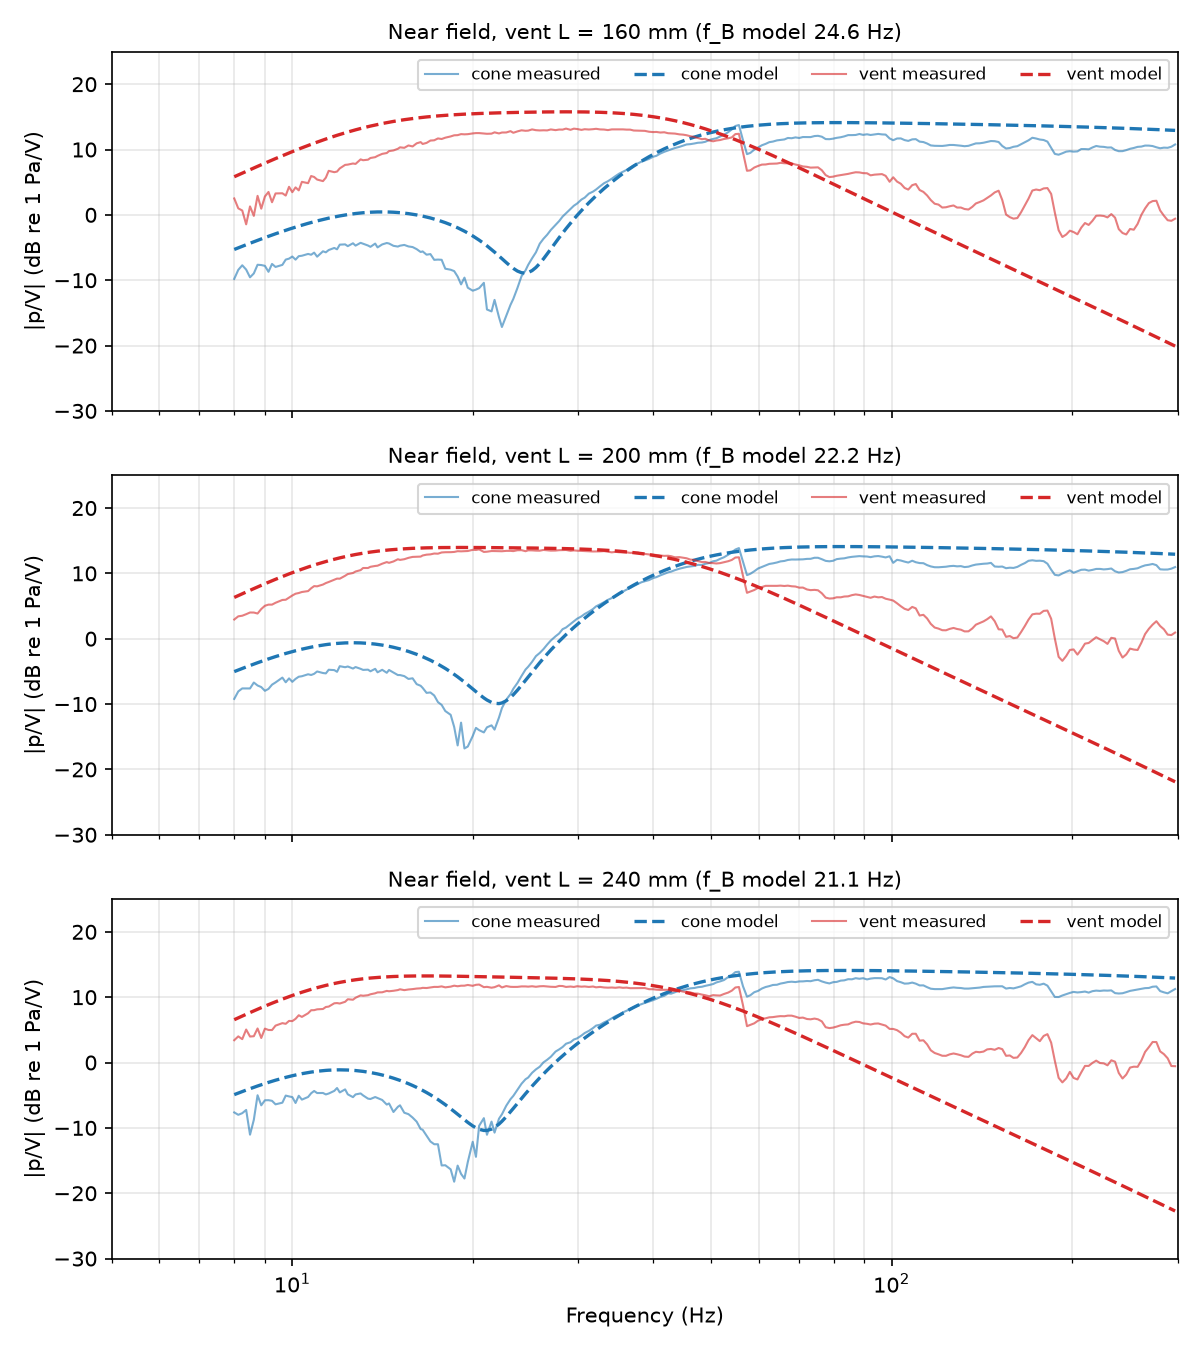
\includegraphics[width=0.85\linewidth]{task1_nearfield.png}
\caption{Near field of cone and vent, measured (Lab D) and predicted by the circuit. Not fitted.}\label{fig:nf}
\end{figure}

\begin{figure}[p]
\centering
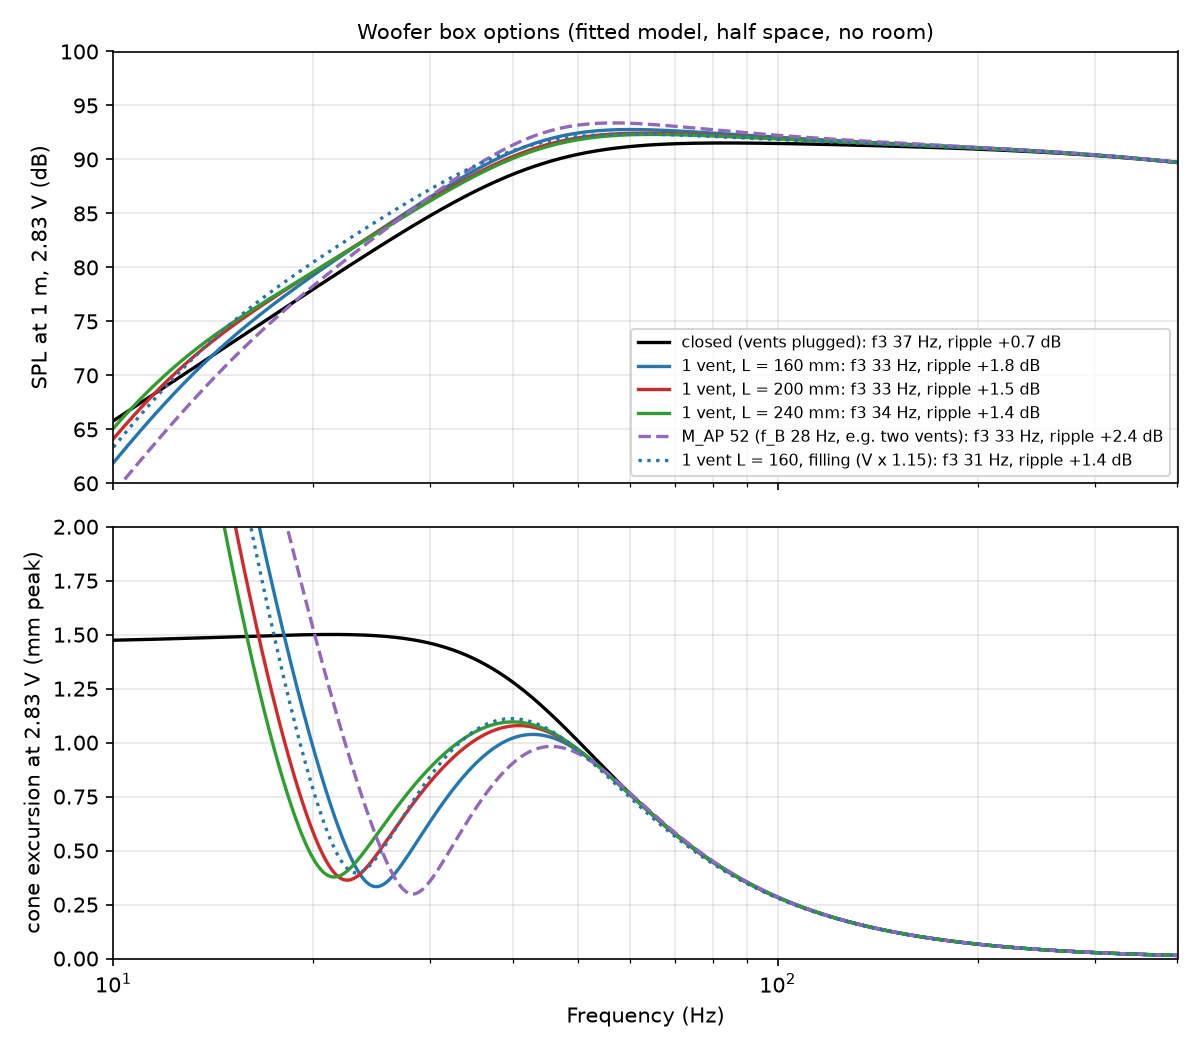
\includegraphics[width=0.85\linewidth]{task1_tuning.png}
\caption{Box options: response at \SI{1}{m} (half space, \SI{2.83}{V}) and cone excursion.}\label{fig:tuning}
\end{figure}

\begin{figure}[p]
\centering
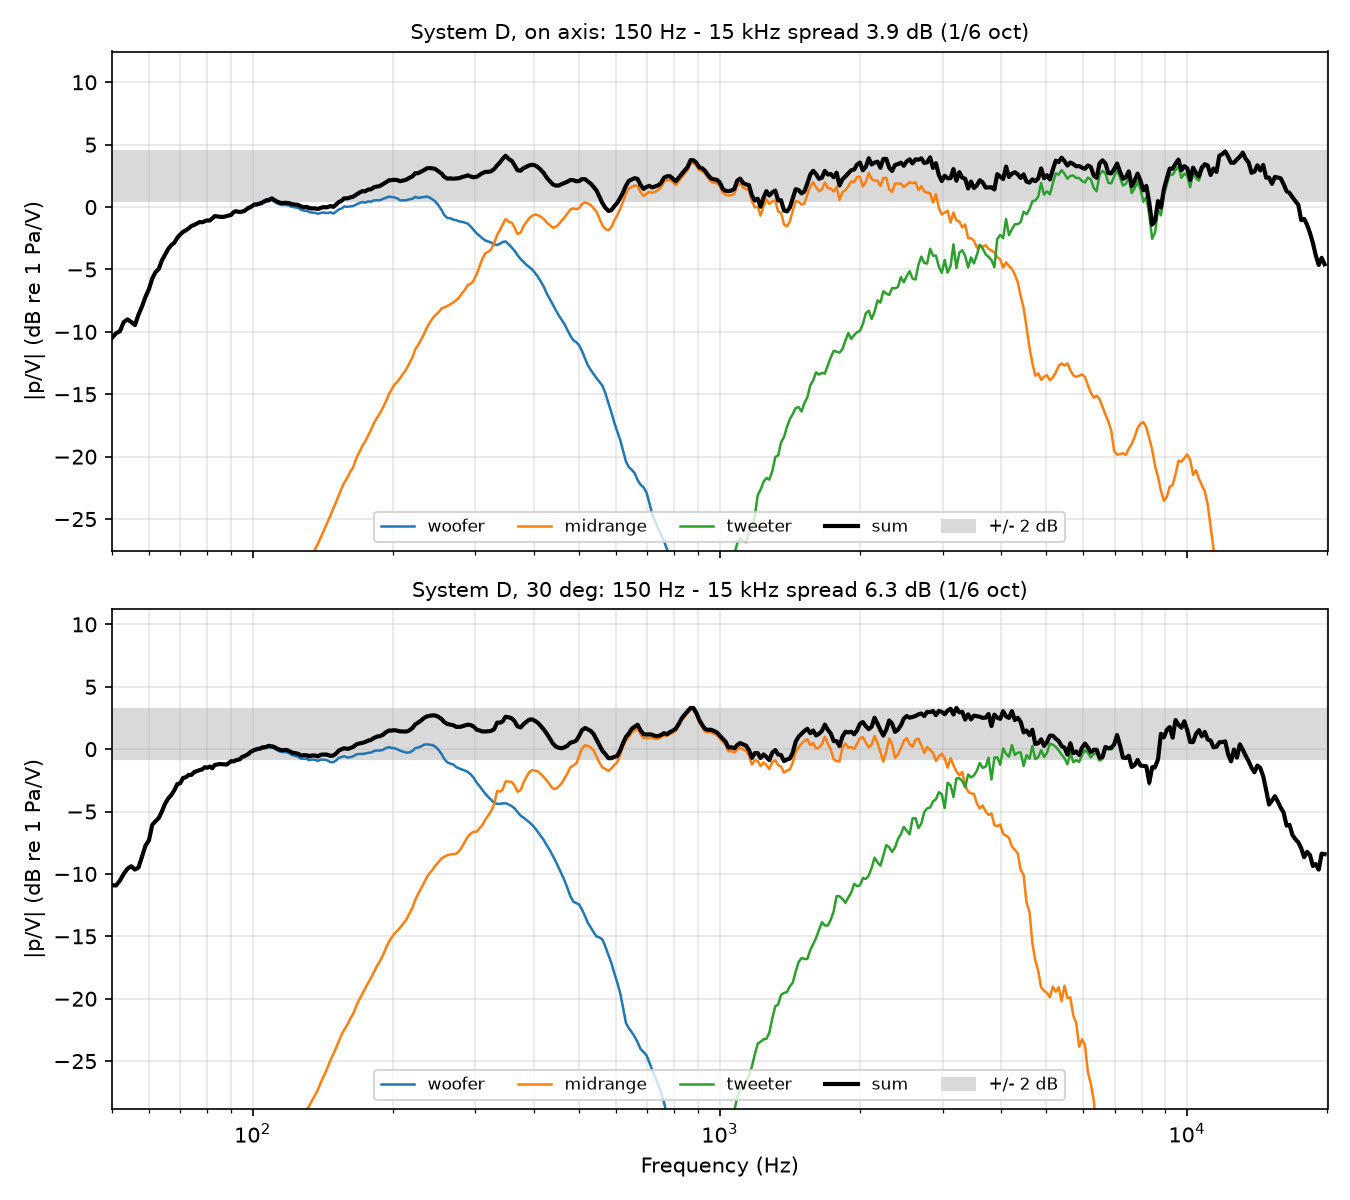
\includegraphics[width=0.9\linewidth]{xover_system.png}
\caption{System response from the measured data: woofer, midrange, tweeter and sum, on axis and at $30^\circ$.}\label{fig:system}
\end{figure}

\begin{figure}[p]
\centering
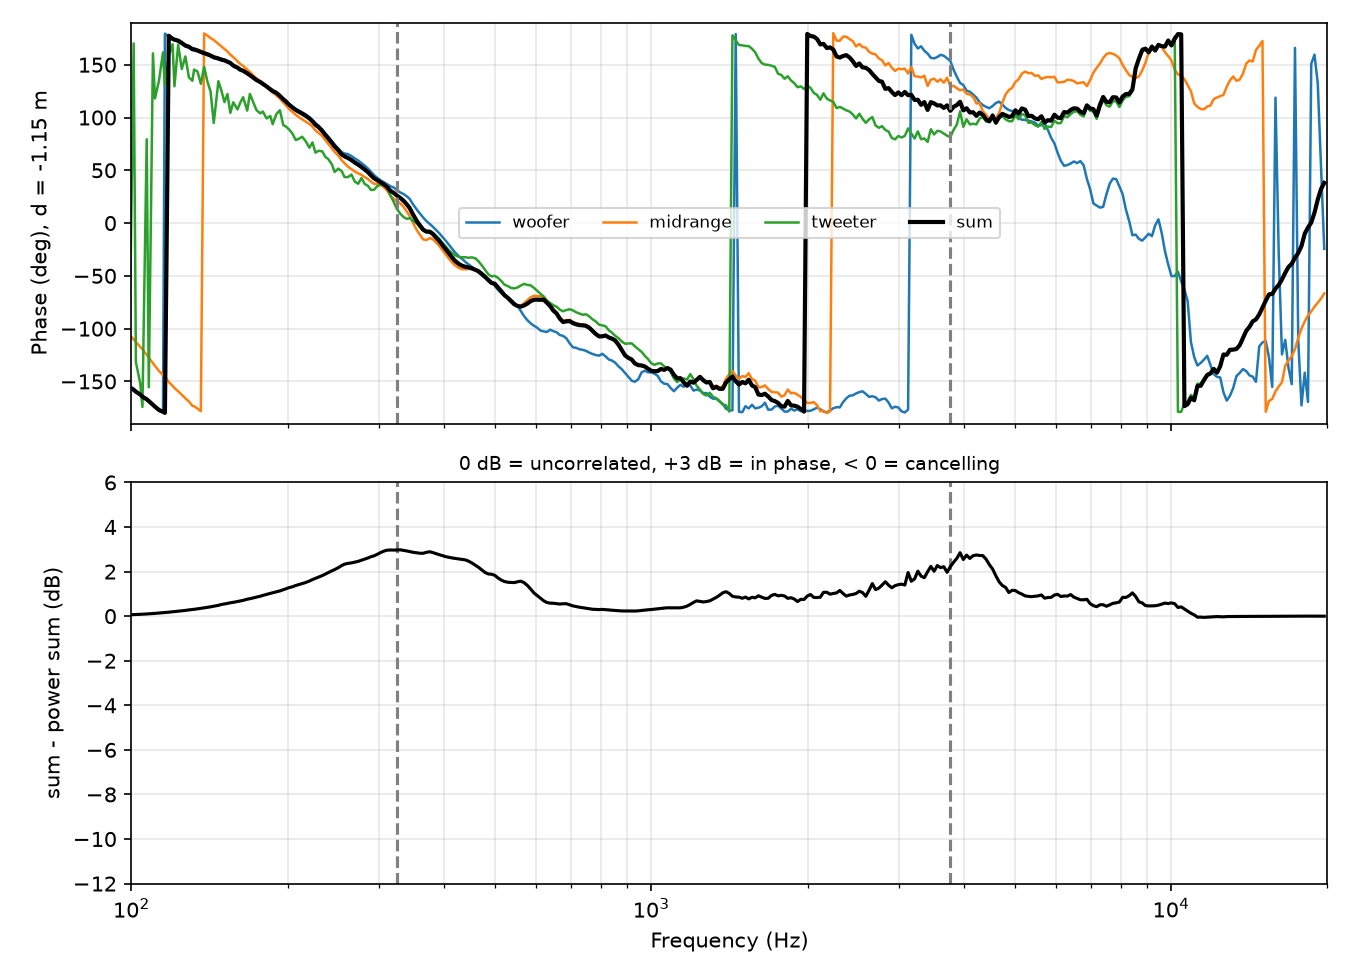
\includegraphics[width=0.9\linewidth]{xover_phase.png}
\caption{Phase of the three contributions ($d = \SI{-1.15}{m}$) and the sum relative to the power
sum: in phase at both crossovers.}\label{fig:phase}
\end{figure}

\begin{figure}[p]
\centering
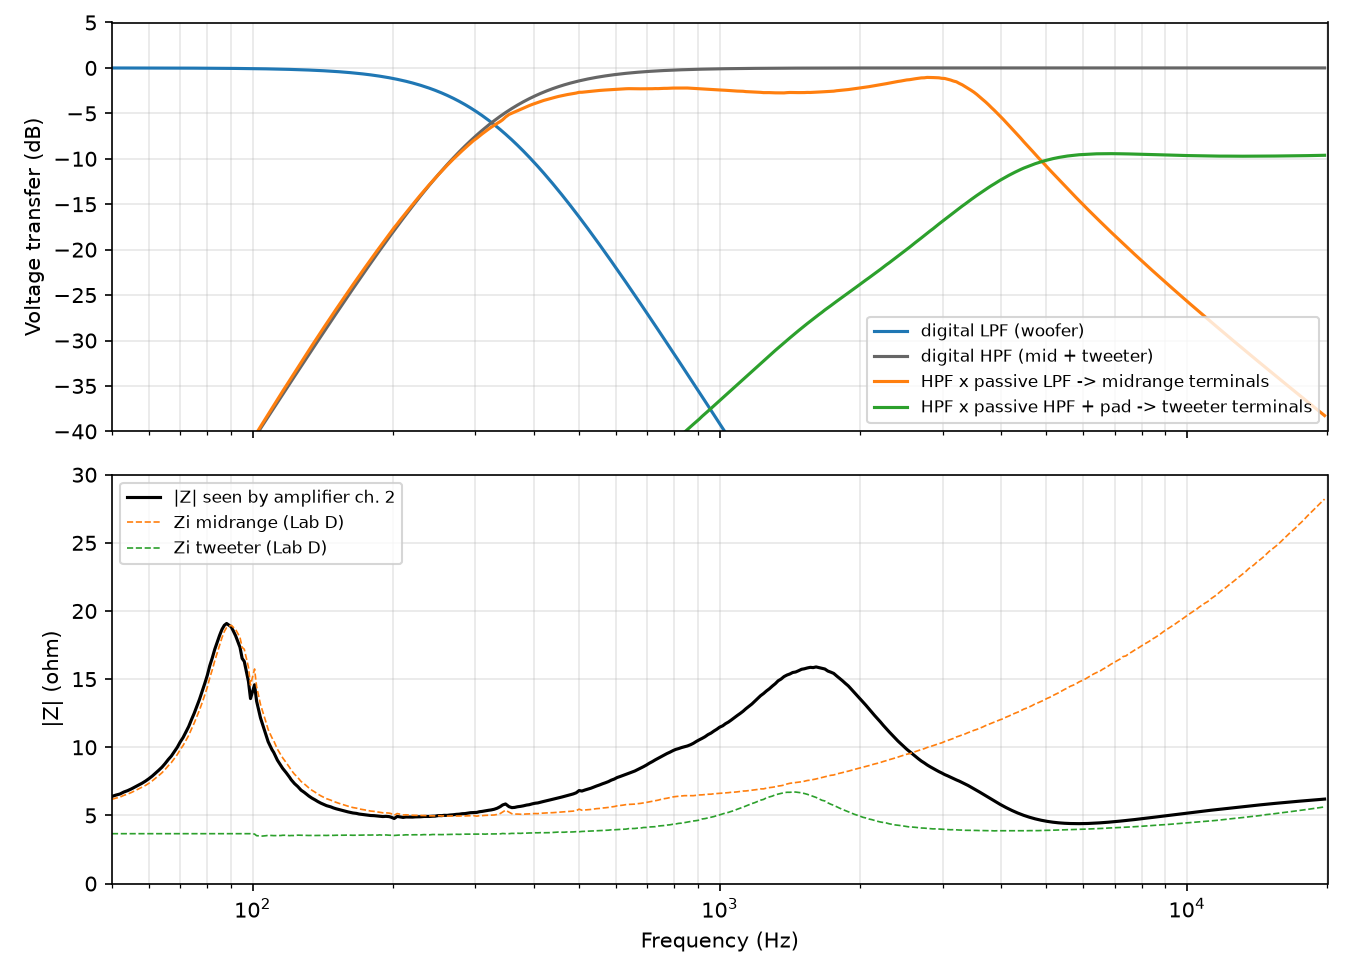
\includegraphics[width=0.9\linewidth]{xover_filters.png}
\caption{Electrical transfer of the digital and passive filters at the driver terminals, and the load
on amplifier channel~2.}\label{fig:filters}
\end{figure}

\begin{figure}[p]
\centering
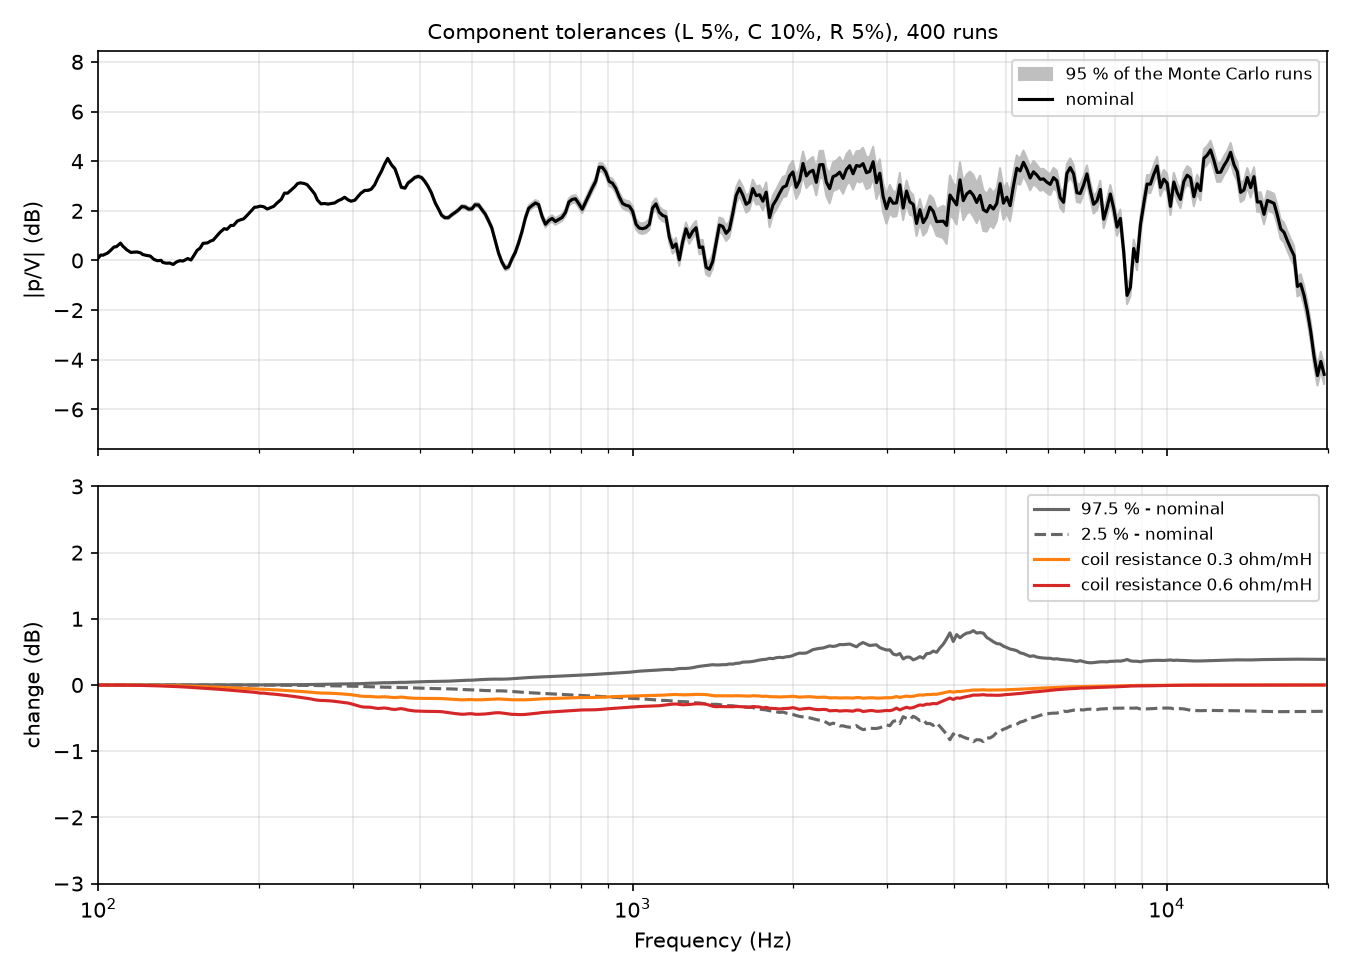
\includegraphics[width=0.9\linewidth]{xover_tolerance.png}
\caption{Component tolerances and coil resistance.}\label{fig:tol}
\end{figure}

\begin{figure}[p]
\centering
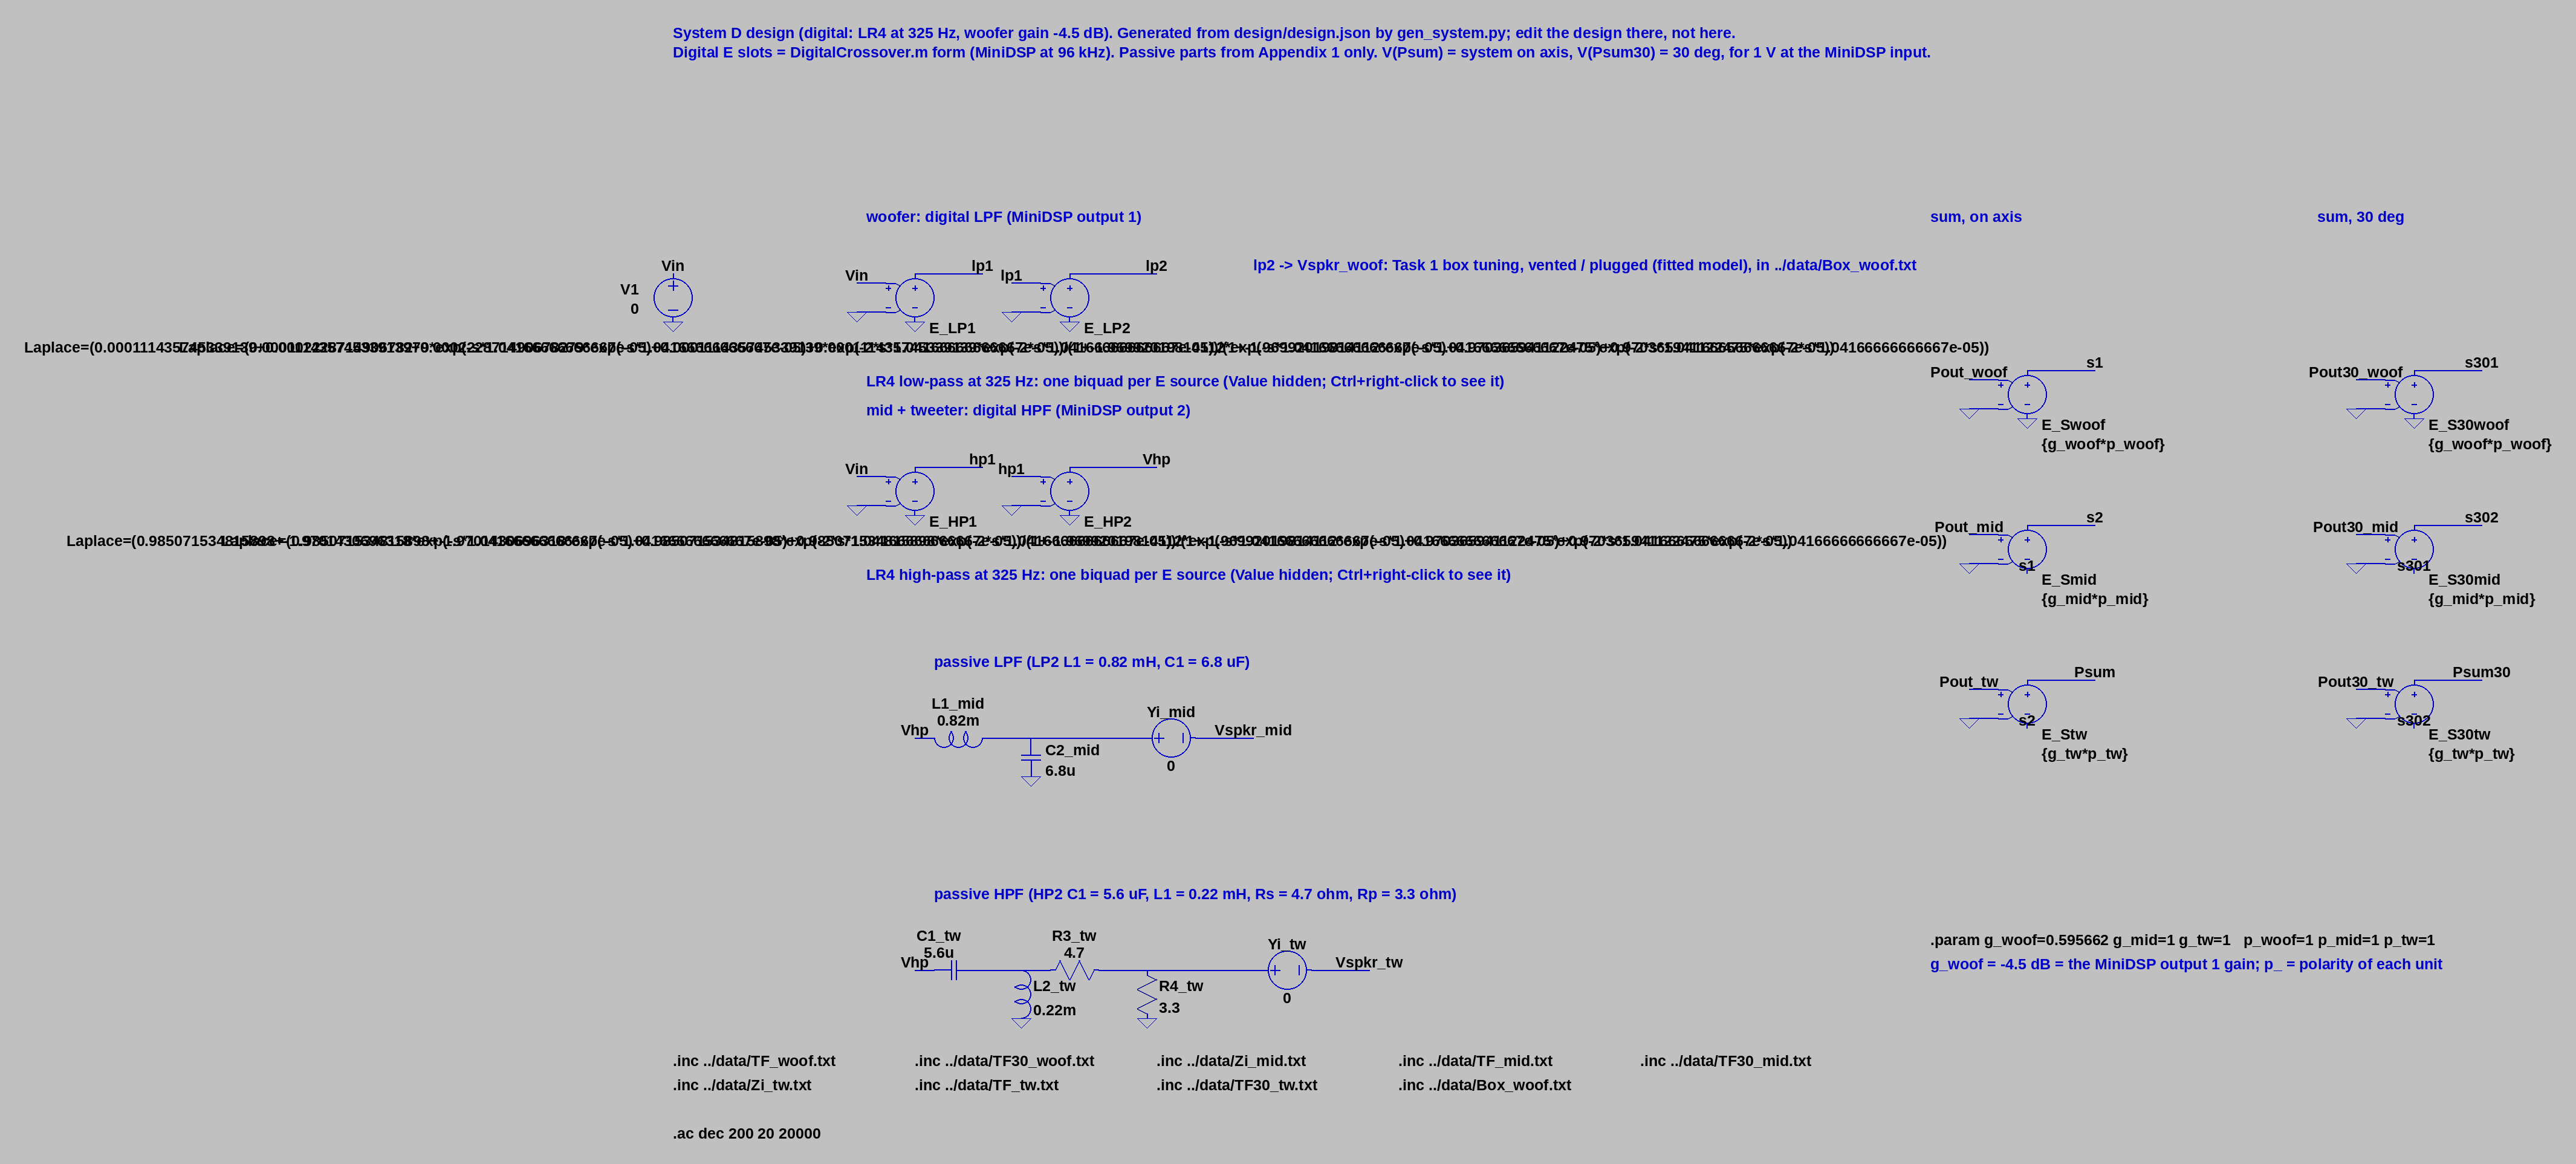
\includegraphics[width=\linewidth]{preview/System_D_design.png}
\caption{\file{System_D_design.asc}: the complete system in LTspice (the long biquad strings are
hidden in LTspice; this rendering shows them).}\label{fig:syssch}
\end{figure}

\end{document}
